\documentclass{article}


\usepackage{arxiv}

\usepackage[utf8]{inputenc} % allow utf-8 input
\usepackage[T1]{fontenc}    % use 8-bit T1 fonts
\usepackage{hyperref}       % hyperlinks
\usepackage{url}            % simple URL typesetting
\usepackage{booktabs}       % professional-quality tables
\usepackage{amsfonts}       % blackboard math symbols
\usepackage{nicefrac}       % compact symbols for 1/2, etc.
\usepackage{microtype}      % microtypography
\usepackage{lipsum}

\usepackage{graphicx}
\graphicspath{ {./images/} }

\title{Proposal: Training Bipedal Robot with Deep Reinforcement Learning}


\author{
  Trey Bean \\
  Udacity Machine Learning Nanodegree\\
  Salt Lake City, UT 84108 \\
  \texttt{trey.bean@icloud.com} \\
}

\begin{document}
\maketitle

% \begin{abstract}
% \lipsum[1]
% \end{abstract}


% keywords can be removed
% \keywords{First keyword \and Second keyword \and More}


\section{Domain Background}
\label{sec:background}
In the world of robotics, programming an computer-based agent to make actions by the use of a rules-based system is tedious, complex, and error-prone. In order to control the robot, programmers would directly control the specific movements, rotations, and positions of each segment and joint of the robot to complete the given task. Not only is this a cumbersome project, it is not very adaptable to handle states that weren't accounted for by the agent's designer or easy to modify it to handle different, yet similar, tasks. In the last decade or so, though, advances in machine learning and specifically deep learning, have made it possible for robotics engineers to focus less on controlling the individual components of a robot, but to instead create programs that learn how to manipulate those components to achieve a given task. While reinforcement learning has been applied to robotics, in the past, the challenge of handling continuous state and action spaces made early attempts at real-world robotics challenges fail to reach much practicality. Adding deep learning to the mix, though, has allowed engineers to overcome these challenges and made the dream of things like self-driving cars and other similar-styled robots almost a reality. 

Personally, I love the problems that machine learning is allowing us to solve. However, many of those problems, e.g. spam detection, language translation, image classification, are things we interface only through a computer or electronic devices. In order to interpret and manipulate the real-world, though, we need robots to facilitate that. I have many things that I wish I could build a robot for, e.g. things as simple as a dandelion-pickers to more complex robots that crawl landfills discovering recyclable and reusable material. In the past, I've known how to construct they physical robots, but have been blocked by how to program them. With Deep Reinforcement Learning agents, though, I'm excited to finally be able to bring some of these ideas to reality.


\section{Problem Statement}
\label{sec:problem}

\begin{figure}[h]
\caption{Bipedal walker falling after taking random actions}
\centering
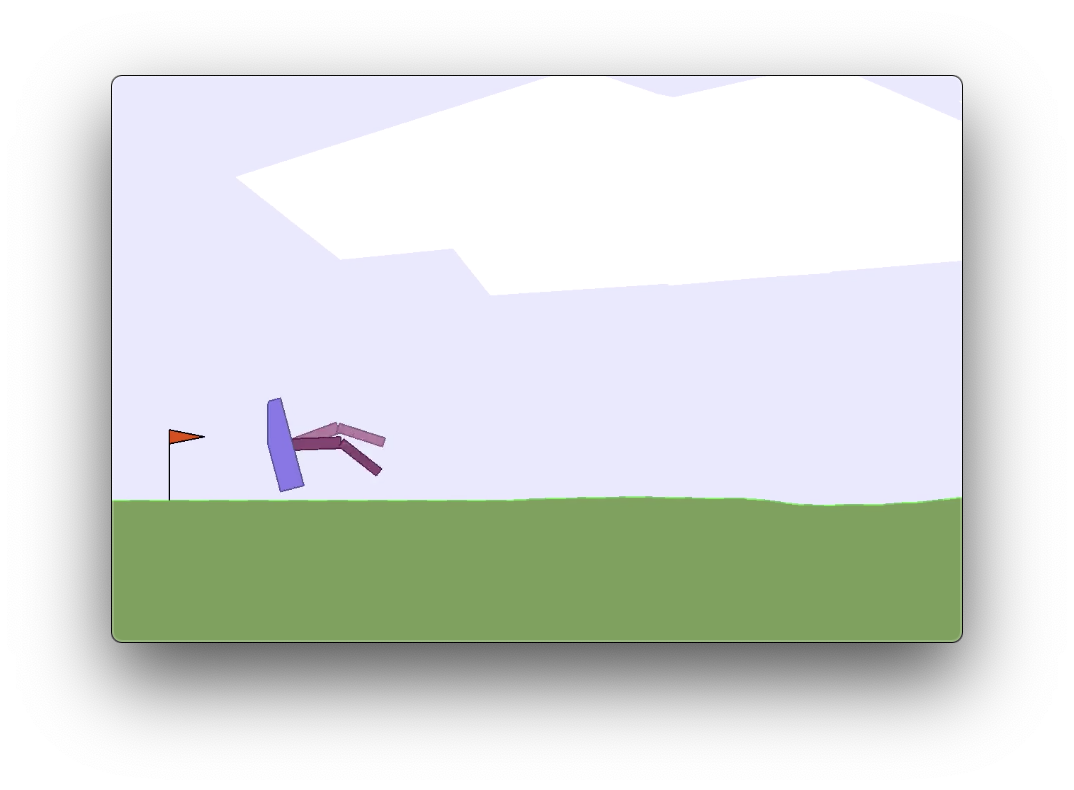
\includegraphics[scale=0.25]{images/bipedal-fall-backward.png}
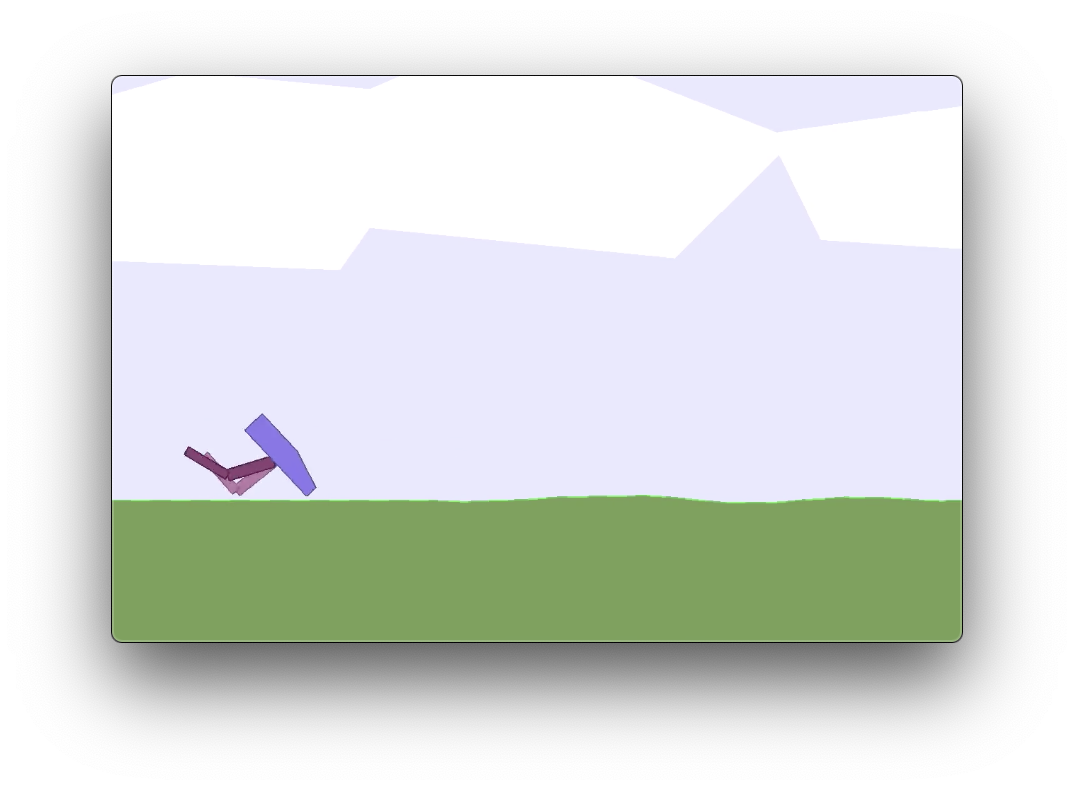
\includegraphics[scale=0.25]{images/bipedal-fall-forward.png}
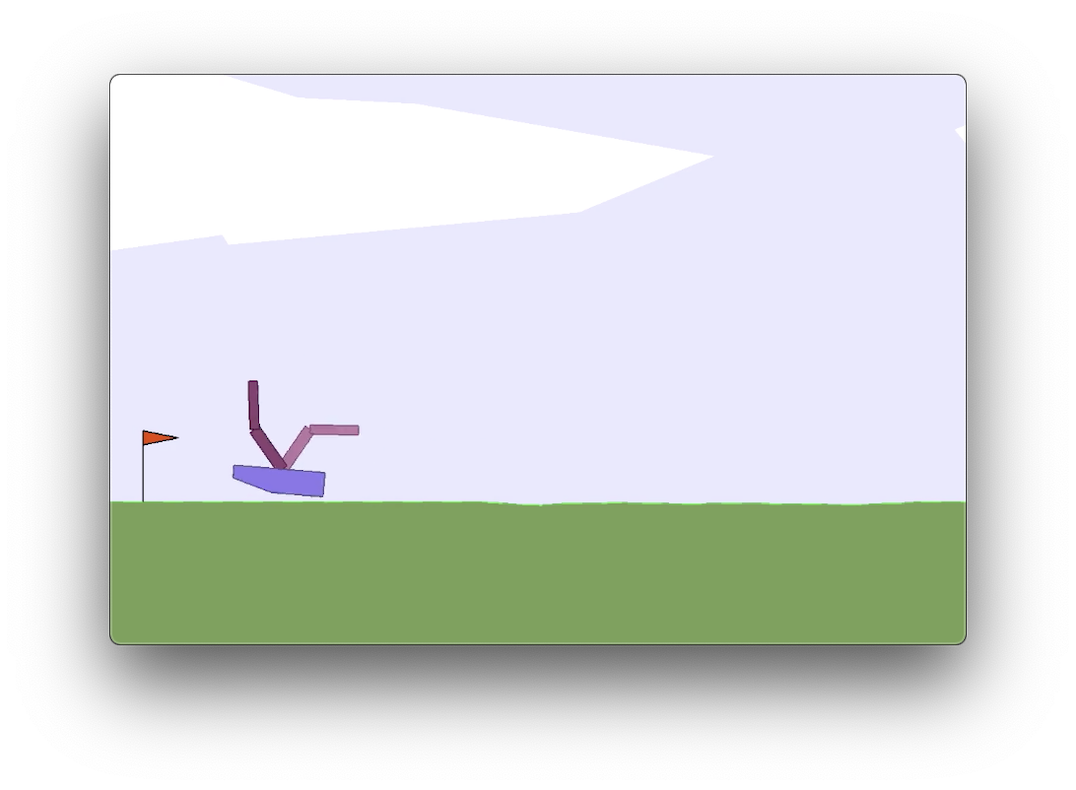
\includegraphics[scale=0.25]{images/bipedal-fall-upside-down.png}
\end{figure}

Specifically, I will be aiming to solve the BipedalWalker-v2 environment that is part of the Box2D environments on OpenAI's Gym. This environment consists of a 4-joint walker robot that is given positive reward for moving, "walking", forward. Solving is defined by OpenAI as averaging a total 300 points in 100 consecutive episodes or trials. While creating an agent that can solve the problem is the primary goal, there is a leaderboard on OpenAI that is ranked by number of episodes required before the agent solves the problem. I will compare my agent against existing results, aiming for a top result.

\section{Datasets and Inputs}
\label{sec:datasets}


(approx. 2-3 paragraphs)

In this section, the dataset(s) and/or input(s) being considered for the project should be thoroughly described, such as how they relate to the problem and why they should be used. Information such as how the dataset or input is (was) obtained, and the characteristics of the dataset or input, should be included with relevant references and citations as necessary It should be clear how the dataset(s) or input(s) will be used in the project and whether their use is appropriate given the context of the problem.


\section{Solution Statement}
\label{sec:solution}
(approx. 1 paragraph)

In this section, clearly describe a solution to the problem. The solution should be applicable to the project domain and appropriate for the dataset(s) or input(s) given. Additionally, describe the solution thoroughly such that it is clear that the solution is quantifiable (the solution can be expressed in mathematical or logical terms) , measurable (the solution can be measured by some metric and clearly observed), and replicable (the solution can be reproduced and occurs more than once).


\section{Benchmark Model}
\label{sec:benchmark}
(approximately 1-2 paragraphs)

In this section, provide the details for a benchmark model or result that relates to the domain, problem statement, and intended solution. Ideally, the benchmark model or result contextualizes existing methods or known information in the domain and problem given, which could then be objectively compared to the solution. Describe how the benchmark model or result is measurable (can be measured by some metric and clearly observed) with thorough detail.


\section{Evaluation Metrics}
\label{sec:metrics}
(approx. 1-2 paragraphs)

In this section, propose at least one evaluation metric that can be used to quantify the performance of both the benchmark model and the solution model. The evaluation metric(s) you propose should be appropriate given the context of the data, the problem statement, and the intended solution. Describe how the evaluation metric(s) are derived and provide an example of their mathematical representations (if applicable). Complex evaluation metrics should be clearly defined and quantifiable (can be expressed in mathematical or logical terms).


\section{Project Design}
\label{sec:design}
(approx. 1 page)

In this final section, summarize a theoretical workflow for approaching a solution given the problem. Provide thorough discussion for what strategies you may consider employing, what analysis of the data might be required before being used, or which algorithms will be considered for your implementation. The workflow and discussion that you provide should align with the qualities of the previous sections. Additionally, you are encouraged to include small visualizations, pseudocode, or diagrams to aid in describing the project design, but it is not required. The discussion should clearly outline your intended workflow of the capstone project.


\bibliographystyle{unsrt}  
\bibliography{references}  %%% Remove comment to use the external .bib file (using bibtex).
%%% and comment out the ``thebibliography'' section.


%%% Comment out this section when you \bibliography{references} is enabled.
% \begin{thebibliography}{1}

% \bibitem{kour2014real}
% George Kour and Raid Saabne.
% \newblock Real-time segmentation of on-line handwritten arabic script.
% \newblock In {\em Frontiers in Handwriting Recognition (ICFHR), 2014 14th
%   International Conference on}, pages 417--422. IEEE, 2014.

% \bibitem{kour2014fast}
% George Kour and Raid Saabne.
% \newblock Fast classification of handwritten on-line arabic characters.
% \newblock In {\em Soft Computing and Pattern Recognition (SoCPaR), 2014 6th
%   International Conference of}, pages 312--318. IEEE, 2014.

% \bibitem{hadash2018estimate}
% Guy Hadash, Einat Kermany, Boaz Carmeli, Ofer Lavi, George Kour, and Alon
%   Jacovi.
% \newblock Estimate and replace: A novel approach to integrating deep neural
%   networks with existing applications.
% \newblock {\em arXiv preprint arXiv:1804.09028}, 2018.

% \end{thebibliography}


\end{document}
